\documentclass[a4paper, 10pt, twocolumn]{article}
\usepackage{amssymb}
\usepackage{cellspace, graphicx, makecell}
\usepackage{graphicx} % Required for inserting images
\usepackage[utf8]{inputenc}
\usepackage[T2A]{fontenc}
\usepackage[english,russian]{babel}
\usepackage{cmap}
\usepackage[left=1cm,right=1cm,
    top=1cm,bottom=2cm]{geometry}
\usepackage{paracol}
\usepackage{multicol}
\usepackage{amsmath}
\usepackage{lipsum}
\usepackage{vwcol}
\usepackage{float}

% Установка размера формул
\DeclareMathSizes{10}{10}{10}{10}   % Для основного текста размером 10pt

\title{Лабораторная работа 1.3.3 \\ Измерение вязкости воздуха по течению в тонких трубках}
\author{Матвей Галицын \\ Б01-411}
\date{April 5, 2025}

\setlength{\columnseprule}{0.1pt}
\setlength{\columnsep}{3em}
\raggedbottom
\begin{document}
\maketitle
\newpage{}
\section{Аннотация}
\textbf{Цель работы:} экспериментально исследовать свойства течения газов по тонким трубкам при различных числах Рейнольдса; выявить область применимости закона Пуазейля и с его помощью определить коэффициент вязкости воздуха.\par
	
\textbf{В работе используются:} система подачи воздуха (компрессор, поводящие трубки); газовый счетчик барабанного типа; спиртовой микроманометр с регулируемым наклоном; набор трубок различного диаметра с выходами для подсоединения микроманометра; секундомер.

\section{Теория}
    Рассмотрим движение вязкой жидкости или газа по трубке круглого сечения. При малых скоростях потока движение оказывается ламинарным (слоистым), скорости частиц меняются по радиусу и направлены вдоль оси трубки. С увеличением скорости потока движение становится турбулентным, а слои перемешиваются. При турбулентном движении скорость в каждой точке быстро меняет величину и направление, сохраняется только средняя величина скорости.

    Характер движения газа (или жидкости) в трубке определяется безразмерным числом Рейнольдса:
    \[
        Re = \frac{vr\rho}{\eta}
    \]
    где $v$ -- скорость потока, $r$ -- радиус трубки, $\rho$ -- плотность движущейся среды, $\eta$ -- её вязкость. В гладких трубах круглого сечения переход от ламининарного движения к турбулентному происходит при $Re \approx 1000$.

    При ламинарном течении объем газа $V$, протекающий за время $t$ по трубе длиной $l$, определяется формулой Пуазейля:
    \begin{equation}
        Q = \frac{\pi r^4}{8 \Delta l \eta}(P_1 - P_2)
    \end{equation}
    В этой формуле $P_1 - P_2$ -- разность давлений в двух выбранных сечениях 1 и 2, расстояние между которыми равно $\Delta l$. Величину $Q$ обычно называют расходом. Формула (1) позволяет определять вязкость газа по его расходу.

    Отметим условия, при которых справедлива формула (1). Прежде всего необходимо, чтобы с достаточным запасом выполнялось неравенство $Re < 1000$. Необходимо также, чтобы при течении не происходило существенного изменения удельного объёма газа (при выводе формулы удельный объём считался постоянным). Для жидкости это предположение выполняется практически всегда, а для газа --- лишь в тех случаях, когда перепад давлений вдоль трубки мал по сравнению с самим давлением. В нашем случае давление газа равно атмосферному ($10^3$ см вод. ст.), а перепад давлений составляет не более 10 см вод. ст., т. е. менее 1\% от атмосферного. Формула (1) выводится для участков трубки, на которых закон распределения скоростей газа по сечению не меняется при двидении вдоль потока.
    \begin{figure}[H]
        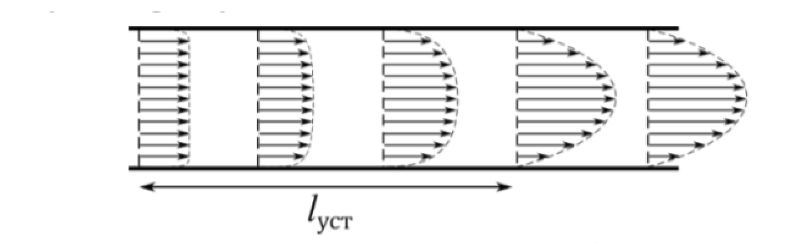
\includegraphics[width=1\linewidth]{images/potok.png}
        \begin{center}
            \caption{Формирование потока газа в трубке круглого сечения}
        \end{center}
    \end{figure}
    При втекании газа в трубку из большого резервуара скорости слоёв вначале постоянны по всему направлению. По мере продвижения газа по трубке картина распределения скоростей меняется, так как сила трения о стенку тормозит прилежащие к ней оси. Характерное для ламинарного течения параболическое распределение скоростей устанавливается на некотором расстоянии $a$ от входа в трубку, которое зависит от радиуса трубки $r$ и числа Рейнольдса по формуле 
    \begin{equation}
        a \approx 0.2rRe
    \end{equation}
    Градиент давления на участке формирования потока оказывается больше, чем на участке с установившимся ламинарным течением, что позволяет разделить эти участки экспериментально. Формула (2) даёт возможность оценить дину участка формирования.

\section{Экспериментальная установка}

    Схема экспериментальной установки изображена на Рис. 2. Поток воздуха
    под давлением, немного превышающим атмосферное, поступает через газовый счётчик в тонкие металлические трубки. Воздух нагнетается компрессором, интенсивность его подачи регулируется краном К. Трубки снабжены
    съёмными заглушками на концах и рядом миллиметровых отверстий, к которым можно подключать микроманометр. В рабочем состоянии открыта заглушка на одной (рабочей) трубке, микроманометр подключён к двум её выводам, а все остальные отверстия плотно закрыты пробками.

    \begin{figure}[H]
        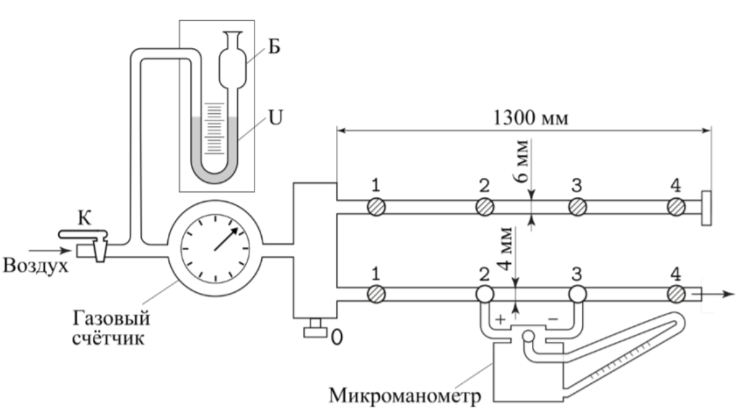
\includegraphics[width=1\linewidth]{images/installation.png}
        \begin{center}
            \caption{Экспериментальная установка}
        \end{center}
    \end{figure}

    Перед входом в газовый счётчик установлен водяной U-образный манометр. Он служит для измерения давления газа на входе, а также предохраняет
    счётчик от выхода из строя. При превышении максимального избыточного
    давления на входе счётчика ($\sim$ 30 см вод. ст.) вода выплёскивается из трубки
    в защитный баллон Б, создавая шум и привлекая к себе внимание экспериментатора.


    \textbf{Газовый счётчик.} В работе используется газовый счётчик барабанного
    типа, позволяющий измерять объём газа $\Delta V$ прошедшего через систему. Измеряя время $\Delta t$ при помощи секундомера, можно вычислить средний объёмный расход газа $Q = \Delta V/ \Delta t$ (для получения массового расхода [кг/с] результат
    необходимо домножить на плотность газа $\rho$).

    \begin{figure}[H]
        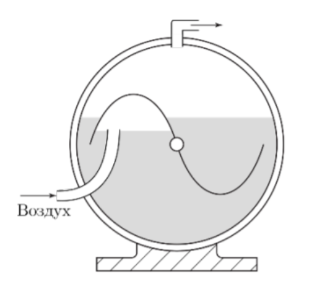
\includegraphics[width=1\linewidth]{images/gasCounter.png}
        \begin{center}
            \caption{Экспериментальная установка}
        \end{center}
    \end{figure}


    Работа счётчика основана на принципе вытеснения: на цилиндрической ёмкости жёстко
    укреплены лёгкие чаши (см. Рис. 3, где для
    упрощения изображены только две чаши), в которые поочередно поступает воздух из входной
    трубки расходомера. Когда чаша наполняется,
    она всплывает и её место занимает следующая
    и т.д. Вращение оси предаётся на счётно-суммирующее устройство.
    Для корректной работы счётчика он должен
    быть заполнен водой и установлен горизонтально по уровню (подробнее см. техническое
    описание установки).

    \textbf{Микроманометр.} В работе используется жидкостный манометр с наклонной трубкой. Разность давлений на входах манометра измеряется по высоте
    подъёма этилового спирта. Регулировка
    наклона позволяет измерять давление в различных диапазонах.

    На крышке прибора установлен трехходовой кран, имеющий два рабочих
    положения — (0) и (+). В положении (0) производится установка мениска жидкости на ноль, что необходимо сделать перед началом работы (в процессе работы также рекомендуется периодически проверять положение нуля). В положении (+) производятся измерения.

\section{Результаты измерений и обработка данных}
    Эксперимент проводился при комнатной температуре $T_\text{комн}=296,2 K$, при атмофсерном давлении $P_\text{атм}=101.99$ кПа.

    Давление, измеряемое микроманометром, определяется по формуле:
    \[
    P=9,81 \cdot K \cdot l 
    \]
    где $l$ -- показание макроманометра, $K$ -- коэффициент наклона, $P$ -- Давление в паскалях.
\subsection{Зависимость разности давлений от расхода}
    Первый эксперимент проводился на трубке с диаметром $d_1 = 3.95\ \pm\ 0,05$ мм. Данные изменрений приведены в табилце № 1.

    Второй эксперимент проводился на трубке с диаметром $d_2 = 5.30\ \pm\ 0,05$ мм. Данные изменрений приведены в табилце № 2.


    С помощью метода наименьших квадратов можно найти коэффициент наклона $Q(\Delta P)$
    $$ k = \frac{\langle Q \cdot \Delta P\rangle}{\langle{\Delta P}^2\rangle} $$
    $$ \Delta k = \frac{1}{\sqrt{n}}\cdot\sqrt{\frac{\langle Q^2 \rangle}{\langle \Delta P^2 \rangle} - k^2}$$
    $$\varepsilon_k = \frac{\Delta k}{k}$$
    Тогда коэффициент вязкости воздуха определяется следующим образом:
    $$ \eta = \frac{\pi \cdot r^4}{8 \cdot \Delta l \cdot k}$$

    Первый эксперимент: 
    $$k_1 = \frac{5800}{2979} \approx 1.94 \frac{\text{мл}}{\text{Па} \cdot c} = 1.94 \cdot 10^{-6} \frac{\text{м}^3}{\text{Па} \cdot c} $$
    $$\Delta k_1 = \frac{1}{\sqrt{9}}\sqrt{\frac{11300}{2979} - 1.94^2} \approx 0.06 \frac{\text{м}^3}{\text{Па} \cdot c} $$
    Аналогично для 2 случая. 
    Соответствующий графиик $Q(\Delta P)$:
    \begin{figure}[H]
        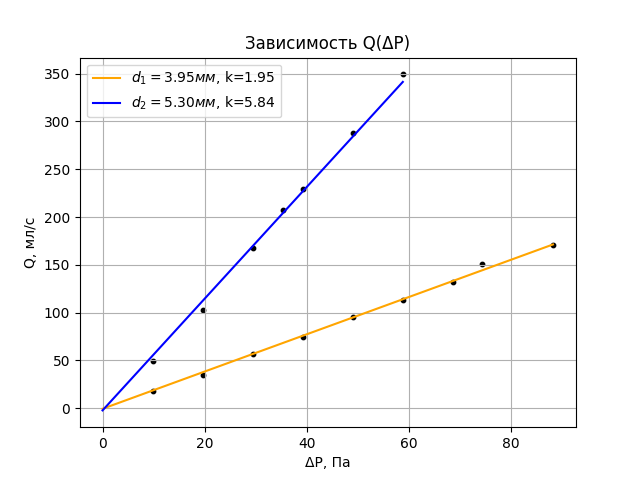
\includegraphics[width=1\linewidth]{graphs/figure1.png}
        \begin{center}
            \caption{$Q(\Delta P)$ (здесь отображены только точки ламинарного течения)}
        \end{center}
    \end{figure}
    Итоговые результаты коэффициента вязкости приведены в таблице № 3.

\subsection{Зависимость разности давлений от длины участка}
\begin{table}[H]
    \centering
    \begin{tabular}{|c|c|c|} \hline
    № & $\Delta x$, cм & $\Delta P$, Па \\ \hline
    \multicolumn{3}{|c|}{$d_1 = 3.95 \text{~мм}, Q = 113.4 \text{мл/c}$} \\ \hline
    1  & 50   & 58.86 \\ \hline
    2  & 40   & 51.01 \\ \hline
    3  & 30   & 37.28 \\ \hline
    4  & 11.2 & 29.43 \\ \hline
    \multicolumn{3}{|c|}{$d_2 = 5.3 \text{~мм}, Q = 287.45 \text{мл/c}$} \\ \hline
    1  & 50   & 49.05 \\ \hline
    2  & 40   & 41.2  \\ \hline
    3  & 30   & 35.32 \\ \hline
    4  & 11.2 & 49.95 \\ \hline
    \end{tabular}
    \caption{Результаты измерений разности давлений от длин участков}
\end{table}
Соответствующий графиик $\Delta P(\Delta x)$:
    \begin{figure}[H]
        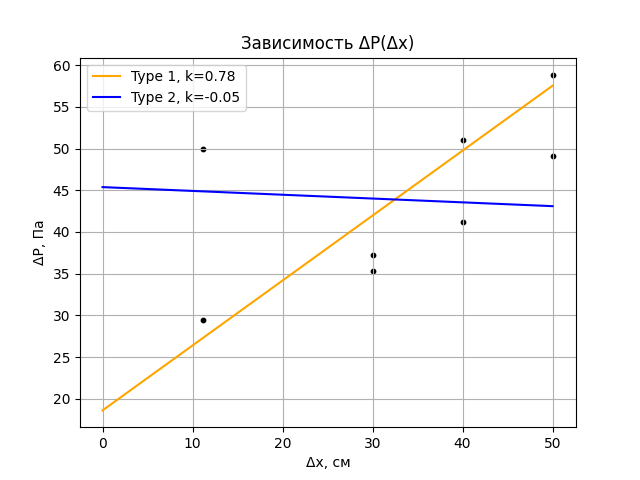
\includegraphics[width=1\linewidth]{graphs/figure2.png}
        \begin{center}
            \caption{$\Delta P(\Delta x)$}
        \end{center}
    \end{figure}
    Исходя из графиков, можно получить критичекую длину трубки $l \approx 30$ см, то есть значительно меньше длины трубки.
    Оценочное число рейнольдса в таком случае $Re \approx 2750$

\subsection{Зависимость расхода от диаметра трубы}
\begin{table}[H]
    \centering
    \begin{tabular}{|c|c|c|c|c|} \hline
    № & $Q, 10^{-6}$ л/с & $r, 10^{-3}$ м & $ln(Q)$ & $ln(r)$ \\ \hline
    \multicolumn{3}{|c|}{Ламинарное течение} \\ \hline
    1  & 95.09   & 3.95 &  \\ \hline
    2  & 287.45  & 5.3 & \\ \hline
    \multicolumn{3}{|c|}{Турбулентное течение} \\ \hline
    1  & 349.87 & 3.95 &  \\ \hline
    2  & 741.35 & 5.3 \\ \hline
    \end{tabular}
    \caption{Результаты измерений разности давлений от длин участков}
\end{table}
    Тогда коэффициент пропорциональности $$\beta = \frac{ln\left(\frac{Q_1}{Q_2}\right)}{ln\left(\frac{R_1}{R_2}\right)}$$
    Получаем:
        $$\beta_{\text{ламинарное}} \approx 3.76   $$
        $$\beta_{\text{турбулентное}} \approx 2.55, $$
    что не плохо согласуется с теорией, согласно которой $\beta_{\text{л}}^{true} = 4$, $\beta_{\text{т}}^{true} = 2.5$.


\section{Обсуждение результатов}
    \begin{itemize}
        \item В ходе исследования анализировалась зависимость свойств течения газа в тонких трубках при различных значениях числа Рейнольдса.
        \item С использованием закона Пуазейля был вычислен коэффициент вязкости воздуха для заданных условий.
        \item Из-за значительных погрешностей полученное значение коэффициента вязкости отклоняется от табличного.
        \item Экспериментально установлено, что при турбулентном течении расход пропорционален \( R^{2,5} \) с высокой точностью.
        \item Для ламинарного течения зависимость расхода оказалась менее точной.
    \end{itemize}
    \newpage
\onecolumn
\section{Приложение}

\begin{table}[H]
    \centering
    \begin{tabular}{|c|c|c|c|c|c|c|c|c|} \hline
    № & $h$, мм & $\Delta V,$ л& $ \Delta t,$ с& $\Delta P$, Па & $Q, $ мл/с & $\Delta P^2, \text{Па}^2$ & $Q, \text{(мл/с)}^2$ & $\Delta P \cdot Q, \frac{\text{мл} \cdot \text{Па}}{\text{с}}$ \\ \hline
    1  & 5  & 1.07  & 60.40 & 9.81  & 17.72  & 96.24   & 313.9  & 173.8   \\ \hline
    2  & 10 & 2.55  & 72.51 & 19.61 & 35.17  & 384.16  & 1236.9 & 689.68  \\ \hline
    3  & 15 & 3.51  & 62.20 & 29.43 & 56.37  & 866.12  & 3177.6 & 1658.9  \\ \hline
    4  & 20 & 4.52  & 60.64 & 39.24 & 74.54  & 1539.78 & 5556.2 & 2924.94 \\ \hline
    5  & 25 & 5.92  & 62.26 & 49.05 & 95.09  & 2405.90 & 9042.1 & 4664.16 \\ \hline
    6  & 30 & 6.88  & 60.67 & 58.86 & 113.40 & 3464.50 & 12859  & 6674.7  \\ \hline
    7  & 35 & 8.01  & 60.62 & 68.67 & 131.99 & 4715.57 & 17421  & 9057.6  \\ \hline
    8  & 40 & 9.13  & 60.41 & 74.48 & 151.13 & 5547.27 & 22840  & 11256.2 \\ \hline
    9  & 45 & 10.33 & 60.40 & 88.29 & 171.03 & 7795.12 & 29251  & 15100.2 \\ \hline
    \shortstack{Среднее \\ знач.} & & & & & & 2979 & 11300 & 5800 \\ \hline
    \multicolumn{6}{|c|}{\text{Турбулентность}}                              \\ \hline
    10 & 55  & 12.59  & 60.63 & 107.91 & 207.65       \\ \hline
    11 & 65  & 14.91  & 60.57 & 127.53 & 246.36                              \\ \hline
    12 & 75  & 19.11  & 68.03 & 147.15 & 280.91                              \\ \hline
    13 & 85  & 8.9    & 29.91 & 166.77 & 297.56                              \\ \hline
    14 & 140 & 10.28 & 30.15 & 274.68 & 340.96                               \\ \hline
    15 & 150 & 10.65 & 30.44 & 294.3  & 349.87                               \\ \hline
    16 & 180 & 11.49 & 30.55 & 353.16 & 376.11                               \\ \hline

    \end{tabular}
    \caption{Результаты измерений разности давлений от расхода}
\end{table}

\begin{table}[H]
    \centering
    \begin{tabular}{|c|c|c|c|c|c|} \hline
    № & $h$, мм & $\Delta V,$ л& $ \Delta t,$ с& $\Delta P$, Па & $Q, $ мл/с \\ \hline
    1  & 5  & 1.01  & 20.45 & 9.81  & 49.39                                  \\ \hline
    2  & 10 & 2.18  & 21.32 & 19.61 & 102.25                                 \\ \hline
    3  & 15 & 3.48  & 20.70 & 29.43 & 168.12                                 \\ \hline
    4  & 18 & 4.09  & 19.72 & 35.32 & 207.4                                  \\ \hline
    5  & 20 & 4.82  & 21.03 & 39.24 & 229.2                                  \\ \hline
    6  & 25 & 5.91  & 20.56 & 49.05 & 287.45                                 \\ \hline
    7  & 30 & 7.11  & 20.36 & 58.86 & 349.21                                 \\ \hline
    \multicolumn{6}{|c|}{\text{Турбулентность}}                              \\ \hline
    8  & 35  & 8.16  & 20.46 & 68.67  & 398.83                               \\ \hline
    9  & 75  & 10.27 & 20.49 & 147.15 & 501.22                               \\ \hline
    10 & 95  & 11.75 & 20.56 & 186.39 & 571.5                                \\ \hline
    11 & 115 & 13.02 & 20.66 & 225.63 & 630.2                                \\ \hline
    12 & 135 & 16.94 & 24.56 & 264.87 & 689.74                               \\ \hline
    13 & 155 & 15.22 & 20.53 & 304.11 & 741.35                               \\ \hline
    14 & 175 & 20.06 & 25.23 & 343.35 & 795.09                               \\ \hline
    \end{tabular}
    \caption{Результаты измерений разности давлений от расхода}
\end{table}

\begin{table}[H]
    \centering
    \begin{tabular}{|c|c|c|c|c|c|} \hline
     & $k, 10^{-6} \frac{\text{м}^3}{\text{с} \cdot \text{Па}}$ & $\Delta k, \frac{\text{м}^3}{\text{с} \cdot \text{Па}}$ & $\varepsilon_k, \%$& $\eta, \text{Па}\cdot\text{с}$ & $\Delta \eta, \text{Па}\cdot\text{с}$\\ \hline
     \shortstack{Первый \\ экспер.} & 1.94 & 0.06  & 3.1 & 19.91 & 0.57  \\ \hline
     \shortstack{Второй \\ экспер.} & 5.84 & 0.12  & 3.1 & 18.98 & 0.57 \\ \hline
    \end{tabular}
    \caption{Результаты вязкостей воздуха в случаях $d_1$ и $d_2$}
\end{table}

\end{document}